
\documentclass[aps,prl,reprint]{revtex4-2}
\usepackage{gensymb}
\usepackage{graphicx}
\usepackage{amsmath}
\usepackage{hyperref}
\usepackage{dsfont}
\usepackage{relsize}
\usepackage{wrapfig}
\usepackage{graphicx}
\usepackage{hyperref}
\hypersetup{colorlinks=true, citecolor=blue, urlcolor=blue, linkcolor=blue}


\begin{document}

% Use the \preprint command to place your local institutional report
% number in the upper righthand corner of the title page in preprint mode.
% Multiple \preprint commands are allowed.
% Use the 'preprintnumbers' class option to override journal defaults
% to display numbers if necessary
%\preprint{}

%Title of paper
\title{Speed of Light Lab}

% repeat the \author .. \affiliation  etc. as needed
% \email, \thanks, \homepage, \altaffiliation all apply to the current
% author. Explanatory text should go in the []'s, actual e-mail
% address or url should go in the {}'s for \email and \homepage.
% Please use the appropriate macro foreach each type of information

% \affiliation command applies to all authors since the last
% \affiliation command. The \affiliation command should follow the
% other information
% \affiliation can be followed by \email, \homepage, \thanks as well.
\author{Trevor Smith, Alex Storrer}
\email[]{smith.tr@northeastern.edu}
\homepage[]{https://github.com/trevorm4x/}
%\thanks{}
%\altaffiliation{}
\affiliation{Northeastern University}


\date{\today}

\begin{abstract}
	The refractive indices of several materials were evaluated.
	The refractive index of air was calculated to be 0.99 $\pm$ 0.01,
	slightly lower than the accepted value of 1.00.
	The refractive index of glass was calculated to be 1.49$\pm$0.03 
	in a glass Fiber-Optic cable.
	The accepted value for the refractive index of glass is 1.52,
	slightly higher than the calculated value.
	The refractive index of water was calculated to be 1.34$\pm$ 0.01,
	slightly higher than the accepted value of 1.33.
	An "effective" refractive index of a coaxial cable was also 
	computed to be 1.56$\pm$0.02.
\end{abstract}


\maketitle

% body of paper here - Use proper section commands
% References should be done using the \cite, \ref, and \label commands
\section{Introduction}
% The Introduction should contain 1 or 2 paragraphs.
% Briefly state the physics underlying the experiment
% (what is being tested and why). 
The speed of light is foundational to our understanding of the universe, as it is in
fact not just the speed photons travel at, but rather a universal speed limit. 
However, even though photons do always travel at the speed of light, we can measure 
the net wavefront in a material at lower speeds, due to the absorption and re-emission
of new photons by atoms in a medium. This ``speed of light in a medium" is usually
thought of not as a speed, but as a ratio $v/c=n$, the refractive index. The 
refractive index is so called because light follows Snells law, where its direction
will be refracted proportional to this refractive index depending on the refractive
indeces of the two mediums.\\

It is, however, also useful to think of ``speed of light in a medium" as a speed, 
because the speed of communications in our incredibly connected world is crucial. 
Even electrical signals, governed by the electromagnetic force which is mediated by
photons, propogate through electrical circuits and cables not at the drift speed of
electrons but rather at the speed an electric field propogates through them. A major
advancement in communications, however, came from using photons themselves rather
than electrical signals to communicate over long distances, using Fiber-Optic (FO) 
cables. These cables take advantage of differences in the refractive index of glass
and another material to create total internal reflection of all photons input at the
end of a long and thin glass tube. These cables are capable of transmitting great 
amounts of information in a very thin tube, as, while conductors permit more 
information to flow through them limited by their circumference, FO cables use their
entire cross-sectional area to transmit information. \\

In this lab, we will measure the speed of light (and the effective speed of light) 
through different mediums, in order to calculate refractive index. The core technique
will involve using a laser and a beam splitter to pass two beams through paths of 
very different lengths, collecting the signals on two photodiodes (PD), and measuring
the relative delay of the longer path compared to the shorter one on an 0.5 GHz
oscilloscope. This laser will be triggered on and off with a nonosecond pulse 
generator. All factors: the pulse generator, the beam path lengths, the sample rate,
and the comparison between the two PD input signals for their time delay, will 
introduce sources of uncertainty that must be minimized by careful measurements and
signal processing. \\

The mediums considered will be air, glass (FO cable), and water. The effective 
index of the coax cables connecting the PD and oscilloscope will also be measured.


\section{Apparatus}
% List equipment components (manufacturer, model
% numbers and brief specifications). 

The apparatus consisted of the following.
\begin{itemize}
\item Oscilloscope, Tektronix TDS210
\item OpenChoice Desktop, Oscilloscope Software
\item Optical breadboard
\item Beam splitter, 2 mirrors, focusing lens
\item Focused laser diode
\item 2 Amplified high-speed silicon photodiodes
\item Water-Filled optical cell
\item Fast edge nanosecond pulse generator
\item Fiber Optic Cable with mount
\item BNC cables and male-male BNC connector
\item Spectrometer and Quantum software, Amadeus
\item Jupyter, Python compiler
\end{itemize}

\section{Procedures and Results}

\subsection{Test Pulse, Scope and Laser Diode}
% Briefly describe the experimental procedures (in your own words, but don’t overdo it)
% Discuss calibrations, etc., if required
% Include necessary equations and put them on their own line (number them, e.g. “Eq. (3)”)
% Include plots showing relevant results (label each figure, e.g. “Fig. 3”, with caption).
% Describe what you found (describe what the plot illustrates)
The  fast  edge  nanosecond  pulse  generator  uses  six74AC14 Schmitt Triggers as shown 
in fig. \ref{Schmitt}, hand mounted to a copper circuit board.\\

\begin{figure}[h]
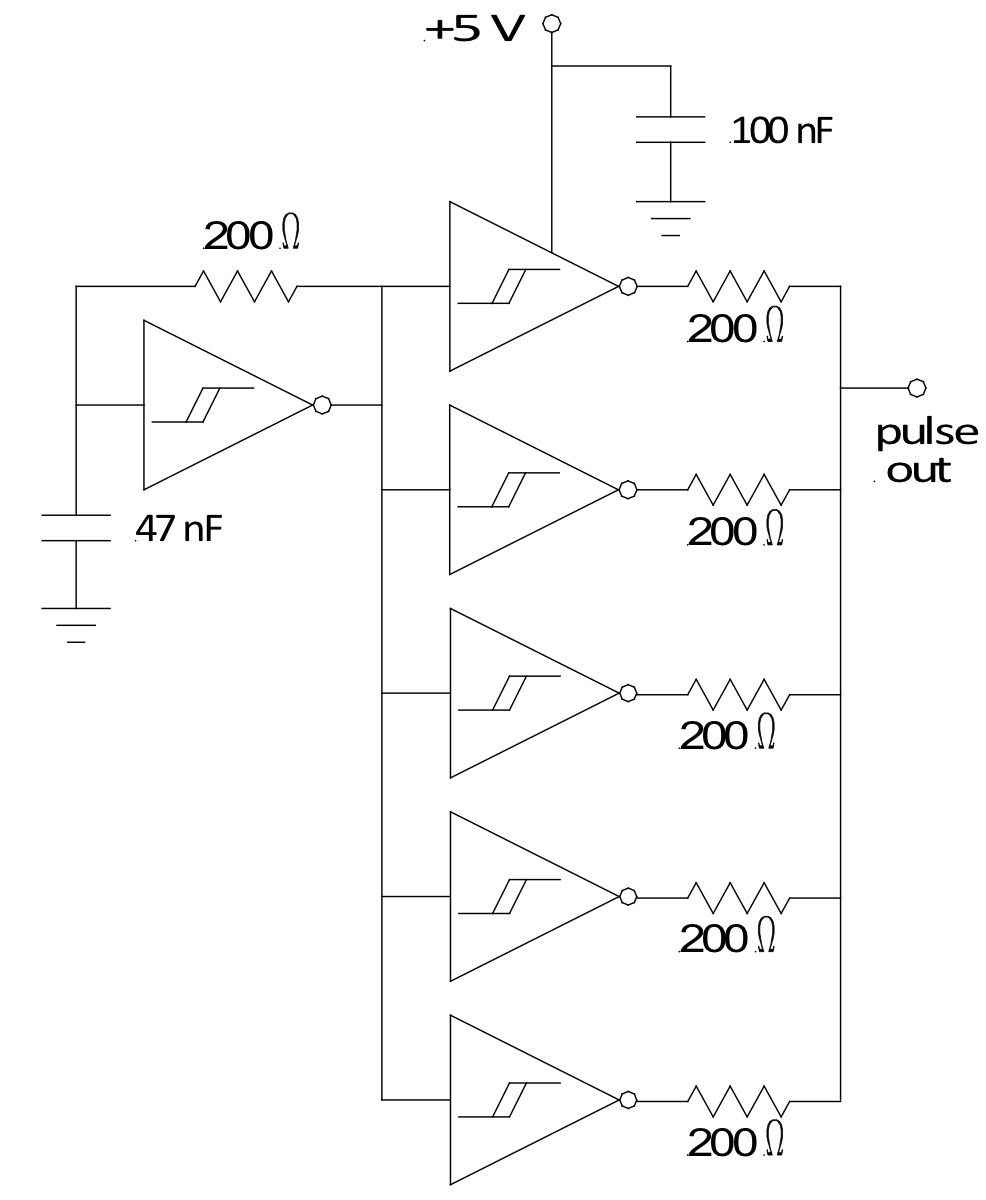
\includegraphics[width=0.4\textwidth]{./BMPs/Schmitt.jpg}
\caption{\label{Schmitt} Circuit diagram of the nanosecond pulse generator}
\end{figure}

The pulse generator was connected directly to the oscilloscope, and adjusted until
several cycles were visible on the display. This output was analyzed to verify the setup.
These square pulses are shown in fig. \ref{squares}. We can observe an approximate 
amplitude of 5.60 mV, and using fourier analysis we can verify that the fundamental 
frequency is 90 kHz. \\

\begin{figure}[h]
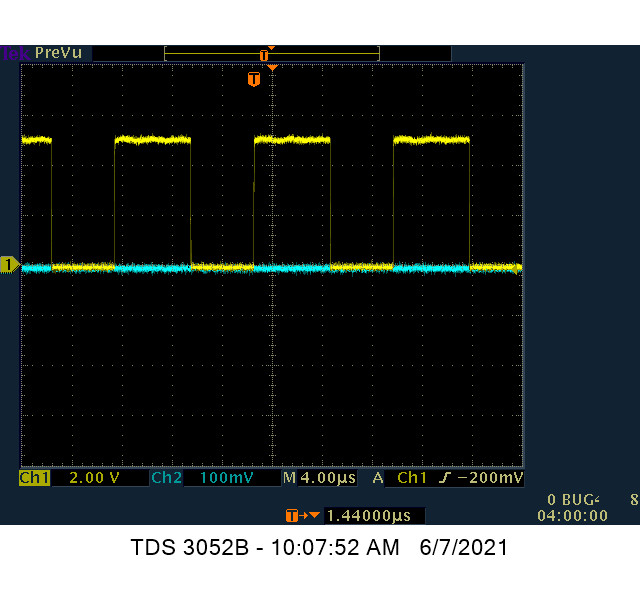
\includegraphics[width=0.4\textwidth]{./BMPs/l4_A_1.jpg}
\caption{\label{squares} Measured square waves on the oscilloscope.}
\end{figure}

The pulse generator will be used to power the laser, creating a wave
front that propogates simultaneously through two paths of different lenghts. \\


\subsection{Optical Setup}

Next, the two paths were configured, based on \ref{setup}. We will consider only the
distances of the paths after the beam splitter, as the paths up until that point are
equivalent. The path measured by PD1 is given by length 1 alone, and the path measured
by PD2 is given by lengths 2-5. These lengths are given in \ref{SetupLengths}, with
all measurements performed with a tape measure.
After completing all measurements in the span of two days,
a final re-demonstration of the lab was performed in a single day, and it is these results
that are shown below, with the geometry of the setup unchanged for the entirety of the 
lab. \\

\begin{figure}[h]
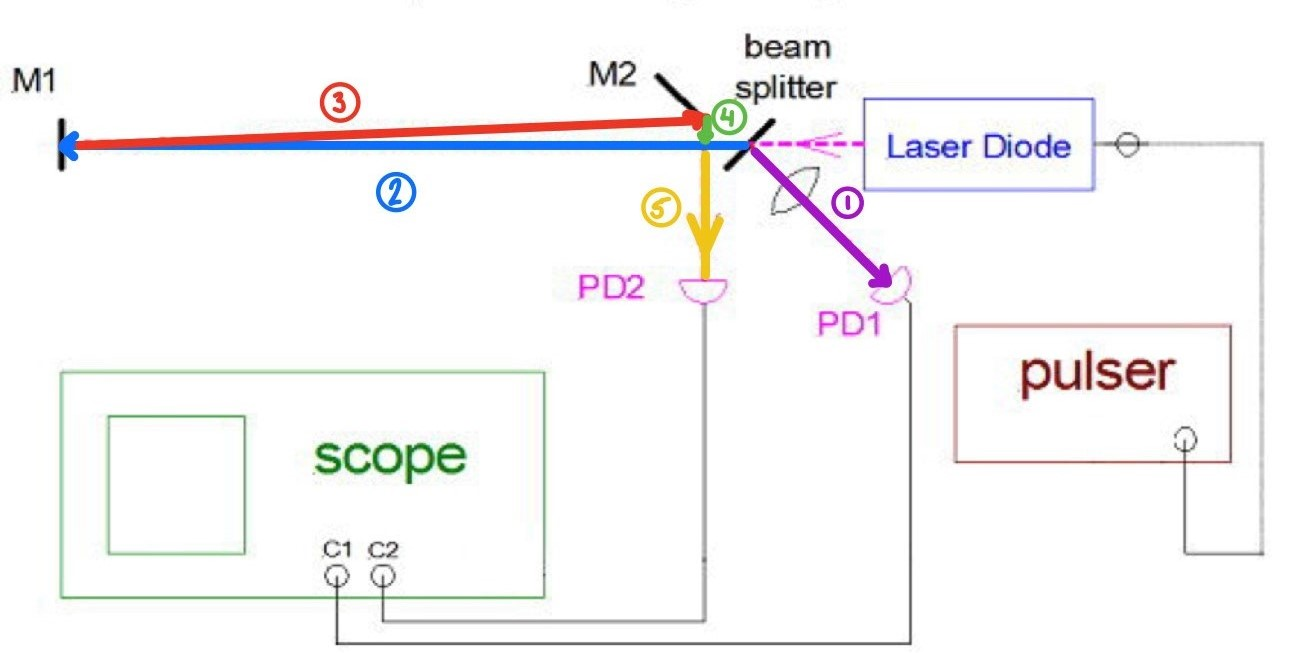
\includegraphics[width=0.4\textwidth]{./BMPs/Optical Setup.jpg}
\caption{\label{setup} Annotated test setup.}
\end{figure}

\begin{table}[h]
\renewcommand{\arraystretch}{1.35}
\setlength{\tabcolsep}{10pt}
\caption{\label{SetupLengths}Lengths of various paths shown the optical setup}
\begin{tabular}{|c|c|c|}
	%\hline
	\toprule
	length \# & Color & Length (mm)\\
	\colrule
	1 & Purple & 168.5\\
	\colrule
	2 & Blue & 917.5\\
	\colrule
	3 & Red & 730.0\\
	\colrule
	4 & Green & 5.0\\
	\colrule
	5 & Mustard & 124.5\\
	\hline
	\botrule
\end{tabular}
\end{table}

Before measuring distances PD1 and PD2 were connected to the oscilloscope, and the signal
was isolated on the oscilloscope, triggered by PD1, as shown in 
\ref{setup}, where a visible time shift can be observed.
By referencing the oscilloscope output, the setup was optimized for the
strongest signal by adjusting the beam splitter and M2. \\

\begin{figure}[h]
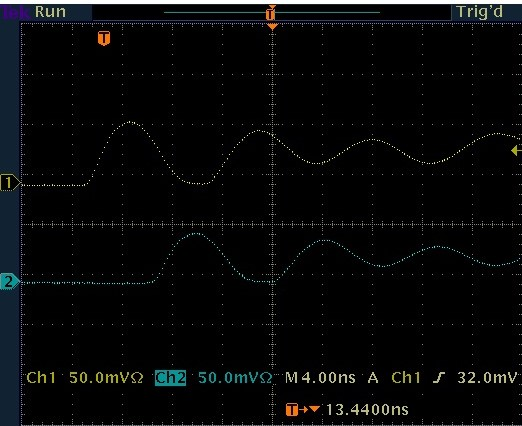
\includegraphics[width=0.45\textwidth]{./BMPs/l4_C_b.jpg}
\caption{\label{setup} Oscilloscope output for test setup with equal length BNC cables.
Signals PD1 and PD2 are labeled on the left 1 and 2 respectively.}
\end{figure}

Measurements were then recorded for analysis, as shown in fig. \ref{same}. It should be
noted that for a perfect experimental setup, these signals would appear as simple step
functions or square waves. However, producing such a sharp signal is very difficult,
and as such more detailed analyis must be done to compare the two signals than simply 
looking at the step time. The ``10-90" rise times were used to compare flight times of 
the two signals, in addition to the min and max of the signals. These values are shown
in table \ref{TD_Ca}. \\

\begin{figure}[h]
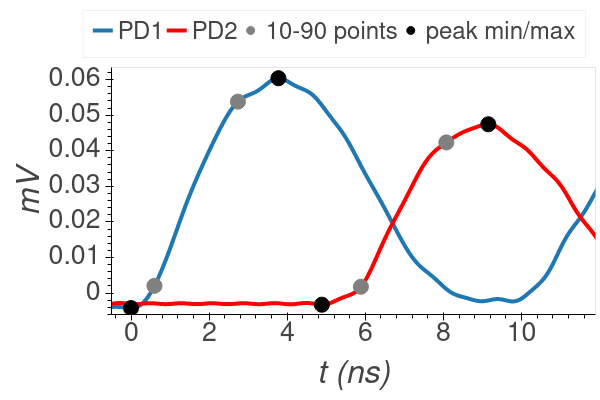
\includegraphics[width=0.45\textwidth]{../Images/l4_C_b.png}
\caption{\label{same} Oscilloscope data comparing reference points for PD1 and PD2.}
\end{figure}

From table \ref{TD_Ca}, the time delay between PD1 and PD2 was calculated, with the
mean and the standard deviation being taken as the recorded measurement and 
uncertainty, at 5.2 $\pm$ 0.2 ns. The high uncertainty in this measurement can
be attributed to the difference in the peak shapes, where the full-width half-max (FWHM)
for PD1 was calculated to be 4.657 ns, and the FWHM for PD2 was calculated to be 4.534 ns.
This error is compensated for in future measurements, but in this case is less relevant. \\

\begin{table}[h]
\renewcommand{\arraystretch}{1.35}
\setlength{\tabcolsep}{10pt}
\caption{\label{TD_Ca}Time values of the first nanosecond peaks for equal length BNC cables}
\begin{tabular}{|c|c|c|c|c|}
%\hline
\toprule
PD & Start & End & 10\% & 90\% \\
\# & (ns)& (ns)& (ns)& (ns)\\
\colrule
1 &    0.0 &  2.47 &  0.67 &  2.02 \\
\colrule
2 &    5.4 &  7.79 &  5.97 &  7.27 \\
\hline
\botrule
\end{tabular}
\end{table}

Next, the BNC cable connecting PD2 to the oscilloscope, which originally was of equal 
length to the cable connecting PD1, was replaced with a significantly longer cable in order
to explore such a scenario, and calculate the effective refractive index of the BNC
cables. The scope output is shown in \fig. \ref{diff}, and the graph with reference points 
included is shown in fig. \ref{setup2}. The values for the 10-90 rise time, min, and max are
shown in table \ref{TD_Cb}. \\


\begin{figure}[h]
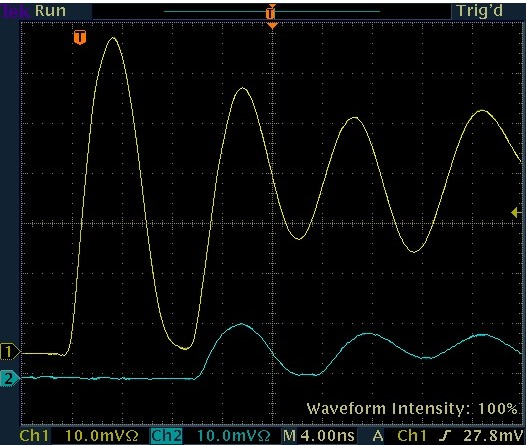
\includegraphics[width=0.45\textwidth]{./BMPs/l4_C_c.jpg}
\caption{\label{setup2} Oscilloscope output for test setup with different length BNC cables.
Signals PD1 and PD2 are labeled on the left 1 and 2 respectively.}
\end{figure}

\begin{figure}[h]
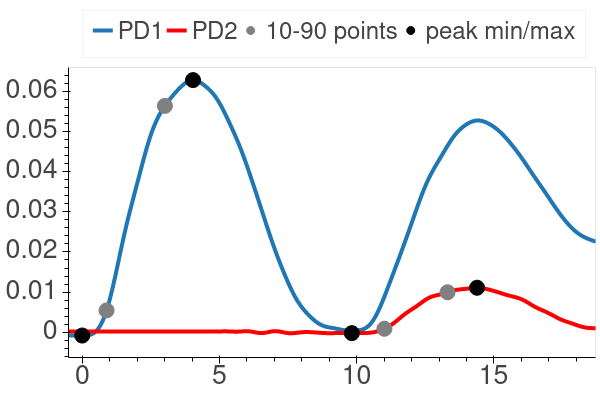
\includegraphics[width=0.45\textwidth]{../Images/l4_C_a.png}
\caption{\label{diff} Oscilloscope data comparing reference points for PD1 and PD2, where PD2 
has been delayed using a longer BNC cable.}
\end{figure}

\begin{table}[h]
\renewcommand{\arraystretch}{1.35}
\setlength{\tabcolsep}{10pt}
\caption{\label{TD_Cb} Time values of the first nanosecond peaks for different length 
	BNC cables}
\begin{tabular}{|c|c|c|c|c|}
%\hline
\toprule
PD & Start & End & 10\% & 90\% \\
\# & (ns)& (ns)& (ns)& (ns)\\
\colrule
1 &   0.00 &   4.04 &   0.89 &   3.01 \\
\colrule
2 &   9.82 &  14.39 &  11.01 &  13.31 \\
\hline
\botrule
\end{tabular}
\end{table}

From table \ref{TD_Cb}, the time delay between PD1 and PD2 with added cable length
was calculated, with the mean and the standard deviation being taken again as the recorded 
measurement and uncertainty, at 10.1 $\pm$ 0.2 ns. This value can be directly compared
to the previous time delay value, as the test setup did not change at all save the cable being 
replaced. By subtracting the time differences for each reference point without added
cable length from the same differences for each reference point with added cable length,
the effect of the cable alone could be isolated. Because of the nature of subtracting
differences of differences, the uncertainty of this resulting measurement was significantly
lower than the previous given values. This value was 4.93 $\pm$ 0.06 ns. \\


A plot showing both sets of captures, with extra
cable and without extra cable, is shown in fig. \ref{comparison}. The extra delay due to
the extra cable length can be seen clearly. \\

\begin{figure}[h]
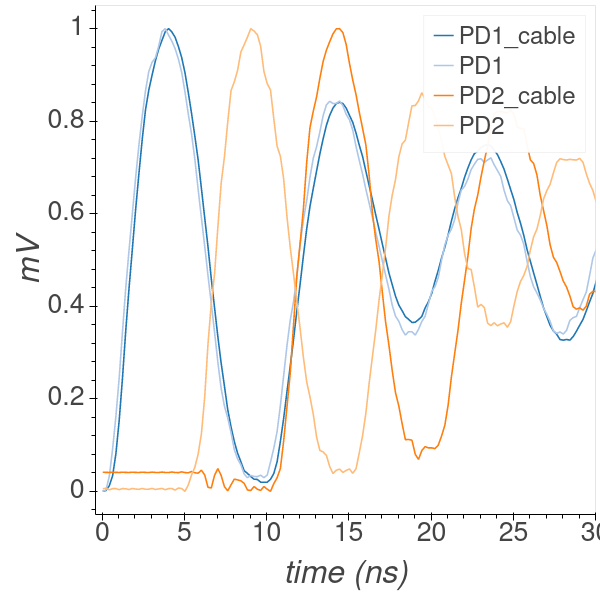
\includegraphics[width=0.45\textwidth]{./l4_A.png}
\caption{\label{comparison} Normalized comparison of the signals from PD1 and PD2 for equal
length cables as well as the inequal length cables, denoted by the suffix ``\_cable".}
\end{figure}

\begin{equation}
	\mathlarger{v = \Delta x/\Delta T}
	\label{vxt}
\end{equation}

Eq. \ref{vxt} was used to calculate the speed of the electric signal in the BNC cable, where
$\Delta x$ is the added distance of cable in meters and $\Delta t$ is the added time delay
in seconds. This speed was found to be $1.92\pm0.02 \times 10^8\ m/s$. The ``effective" 
refractive index was calculated using eq. \ref{duh}, where n is the refractive index, c is
the speed of light in vacuum, and v is the speed of light in a given medium. The effective
refractive index of the BNC cable was calculated to be 1.56 $\pm$ 0.02. \\

It is clear that if one cable was longer than the other then the time delay would be 
substantially altered. In the actual test setup, every part of the setup that both
beams experience is not considered, as it does not factor into the cause of the time
delay between the beams. This includes the path of the beam before it splits, but
also the paths of the electric signals from the PD sensors to the oscilloscope. If
the paths were not the same then this error would completely ruin our ability to
record accurate data. \\

\begin{equation}
	\mathlarger{n=c/v}
	\label{duh}
\end{equation}

\subsection{Speed of Light in Air}

The speed of light in air was found using the same setup as in the previous section, after 
removing the extra length BNC cable. The raw output of the oscilloscope for this step is
shown in fig. \ref{air_osc}. \\

\begin{figure}[h]
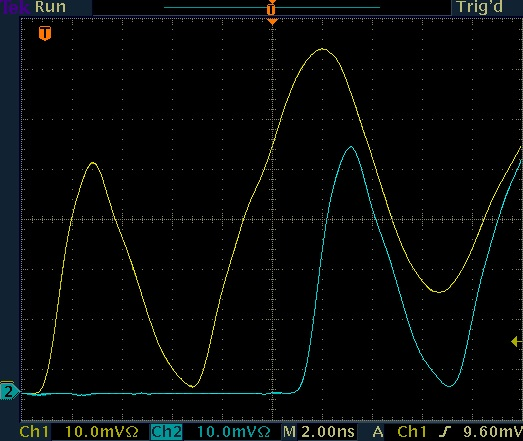
\includegraphics[width=0.45\textwidth]{./BMPs/l4_D_1_a.jpg}
\caption{\label{air_osc} Oscilloscope readout of the two signals PD1 (yellow) and PD2
	(blue) for the two paths in air. }
\end{figure}

Because of the importance of precisely measuring peak times,
some high frequency noise was filtered out with a simple square-cutoff low-pass filter,
and cubic spline interpolation was used to increase measuring precision of the wave 
features. This spline interpolation is justified by the fact that the oscilloscope is
averaging 512 waves in this single observation, improving measurement precision when
projecting curves between points. The processed signal, with all peaks besides the
first ones removed, is shown in fig. \ref{air_boke}. \\

\begin{figure}[h]
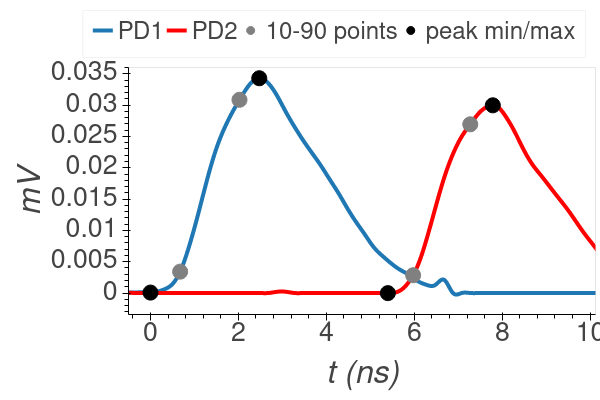
\includegraphics[width=0.45\textwidth]{../Images/l4_D_a.png}
\caption{\label{air_boke} Processed signals PD1 and PD2 in air, with calculated
reference points included.}
\end{figure}

The values for the time shifts with respect to each signal reference point is shown in
Table \ref{TD_D1}. The average and standard deviation of the time shift was found 
to be 5.32 $\pm$ 0.07 ns. By referencing the setup geometry and using eq. \ref{vxt}, the
speed of light in air was calculated to be $3.01 \pm 0.04 \times 10^8\ m/s$, and
by using eq. \ref{duh} the corresponding refractive index was found to be 0.99 $\pm$ 0.01.
The accepted value of 1.0003 is therefore within the uncertainty. This uncertainty
mostly comes from measuring distances with a measuring tape, lining up the markings
on the tape with laser pulses that are below it, however some error also comes from
the length of the nanosecond pulse and the difference in signal shapes between PD1 and PD2. \\

\begin{table}[h]
\renewcommand{\arraystretch}{1.35}
\setlength{\tabcolsep}{10pt}
\caption{\label{TD_D1}Time values of the first nanosecond peaks for equal length BNC cables}
\begin{tabular}{|c|c|c|c|c|}
%\hline
\toprule
PD & Start & End & 10\% & 90\% \\
\# & (ns)& (ns)& (ns)& (ns)\\
\colrule
1 &    0.0 &  2.47 &  0.67 &  2.02 \\
\colrule
2 &    5.4 &  7.79 &  5.97 &  7.27 \\
\hline
\botrule
\end{tabular}
\end{table}




\subsection{Speed of Light in Glass}

The speed of light in glass was found using the same setup as in the previous section,
but the PD2 mount was replaced with a holder for a FO cable, and this FO cable, measured
at 2065.5 $\pm$ 0.5 m was plugged directly into PD2, such that a length of glass cable
was added to the previous setup. The raw output of the oscilloscope for this step is shown in fig. 
\ref{glass_osc}. \\

\begin{figure}[h]
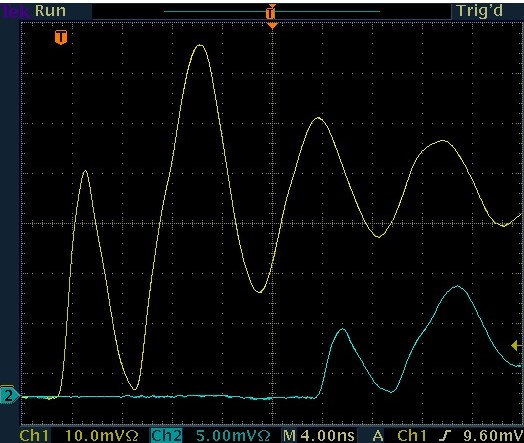
\includegraphics[width=0.45\textwidth]{./BMPs/l4_D_2_a.jpg}
\caption{\label{glass_osc} Oscilloscope readout of the two signals PD1 (yellow) and PD2
	(blue) for the two paths in glass. }
\end{figure}

The same pre-processing as in the previous step was used again.
The processed signal, with all peaks besides the
first ones removed, is shown in fig. \ref{glass_boke}. \\

\begin{figure}[h]
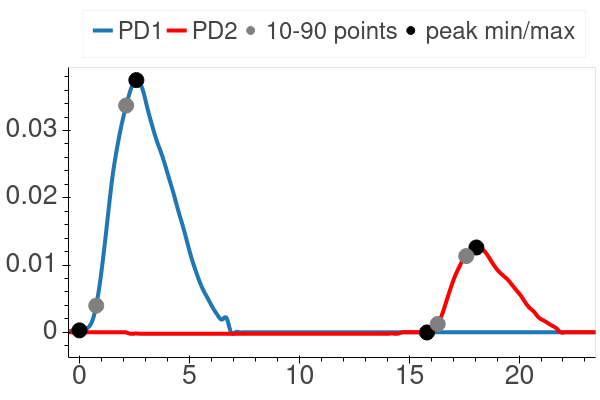
\includegraphics[width=0.45\textwidth]{../Images/l4_D_b.png}
\caption{\label{glass_boke} Processed signals PD1 and PD2 in glass, with calculated
	reference points included.}
\end{figure}

The values for the time shifts with respect to each signal reference point is shown in
Table \ref{TD_D2}. The average and standard deviation of the time shift was found 
to be 15.6 $\pm$ 0.2 ns. In order to account for just the effect of the glass, the previous
value for the time-shift due to air in the prior step was simply subtracted from this one,
giving a 10.3 $\pm$ 0.2 ns time shift due to the FO cable. 
By using the equation for velocity \ref{vxt}, the speed of light in glass was calculated
to be $2.01 \pm 0.03 \times 10^8\ m/s$, and
by using eq. \ref{duh} the corresponding refractive index was found to be 1.49 $\pm$ 0.03.\\

\begin{table}[h]
\renewcommand{\arraystretch}{1.35}
\setlength{\tabcolsep}{10pt}
\caption{\label{TD_D2}Time values of the first nanosecond peaks with an extra FO cable inserted into PD2}
\begin{tabular}{|c|c|c|c|c|}
%\hline
\toprule
PD & Start & End & 10\% & 90\% \\
\# & (ns)& (ns)& (ns)& (ns)\\
\colrule
1 &   0.00 &   2.59 &   0.76 &   2.12 \\
\colrule
2 &  15.81 &  18.06 &  16.30 &  17.60 \\
\hline
\botrule
\end{tabular}
\end{table}

The accepted value of 1.52 is therefore within the uncertainty. Again, this uncertainty
mostly comes from measuring distances with a measuring tape, lining up the markings
on the tape with laser pulses that are below it, however some error also comes from
the length of the nanosecond pulse and the difference in signal shapes between PD1 
and PD2. \\

\subsection{Speed of Light in Water}

The speed of light in water was found using the same setup as in the previous section,
Speed of Light in Air, by placing a clear plastic tube full of water, measuring 
614.0 $\pm$ 0.05 mm, in the PD2 beam path such that the beam would pass through it twice.
Specifically, the tube was placed along paths 2 and 3 in the fig \ref{setup}. Special
care was taken when originally setting up the first experiment to make sure that the
beam traveling along path 2 was 5mm away from the location where path 3 is incident
on M2, specifically for this phase of the test, and as such no measurements were
retaken here.  The raw output of the oscilloscope for this step is shown in fig. 
\ref{water_osc}. \\

\begin{figure}[h]
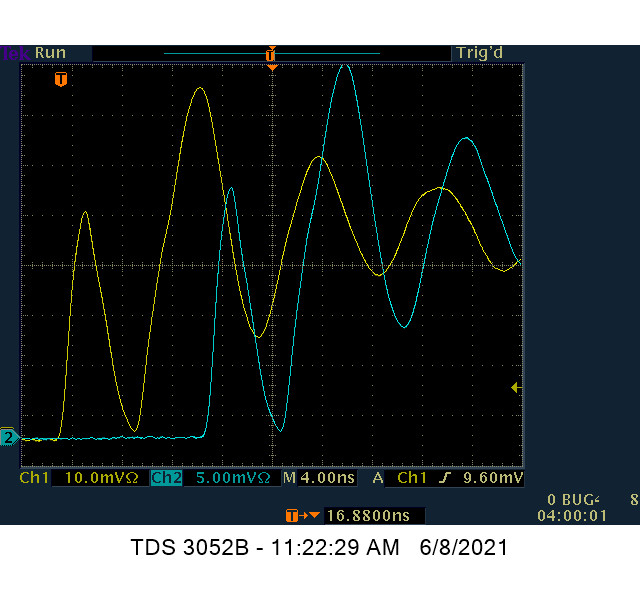
\includegraphics[width=0.45\textwidth]{./BMPs/l4_D_3_a.jpg}
\caption{\label{water_osc} Oscilloscope readout of the two signals PD1 (yellow) and PD2
	(blue) for the two paths in water. }
\end{figure}

The same pre-processing as in the previous step was used again.
The processed signal, with all peaks besides the
first ones removed, is shown in fig. \ref{water_boke}. \\

\begin{figure}[h]
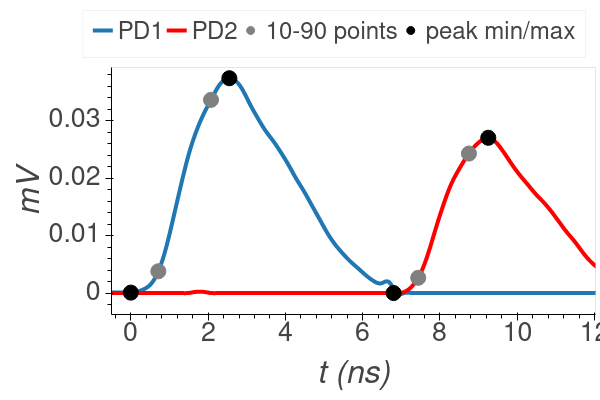
\includegraphics[width=0.45\textwidth]{../Images/l4_D_c.png}
\caption{\label{water_boke} Processed signals PD1 and PD2 in water, with calculated
	reference points included.}
\end{figure}

The values for the time shifts with respect to each signal reference point is shown in
Table \ref{TD_D3}. The calculation of the time-of-flight of light through water in this
test setup is more complex than in the other phases of this experiment because in this
case, water \emph{replaces} air along a portion of the path length for PD2. We can
assume that because the speed of light is constant, we can subtract out the length
the light traveled through air in our water measurement by finding the proportion
of the time-shift in air that is due to the length other than that covered by the water
tube, as shown in eq. \ref{TD_Air3}. 

\begin{equation} 
t_{air delay} = \frac{L_2+L_3+L_4+L_5 - 2L_{water}}{v_{air}}
\label{TD_Air3}
\end{equation}

Where v$_{air}$ is the speed of light in air calculated in the preceding section, L$_2$ to L$_5$ are the path 
lengths in Figure \ref{OpticalSetup}, and L$_{water}$ is the length of the water cell which is multiplied by 2 
since the laser passes through it twice. \\

This value for time-of-flight through the water tube alone was calculated to be 6.72 $\pm$ 0.5 ns. 
By using the equation for velocity \ref{vxt}, the speed of light in glass was calculated
to be $2.24 \pm 0.02 \times 10^8\ m/s$, and
by using eq. \ref{duh} the corresponding refractive index was found to be 1.34 $\pm$ 0.01.\\

\begin{table}[h]
\renewcommand{\arraystretch}{1.35}
\setlength{\tabcolsep}{10pt}
\caption{\label{TD_D3}Time values of the first nanosecond peaks when a water-filled optical cell is in the path leading to PD2}
\begin{tabular}{|c|c|c|c|c|}
%\hline
\toprule
PD & Start & End & 10\% & 90\% \\
\# & (ns)& (ns)& (ns)& (ns)\\
\colrule
1 &    0.0 &  2.55 &  0.71 &  2.07 \\
\colrule
2 &    6.8 &  9.25 &  7.44 &  8.75 \\
\hline
\botrule
\end{tabular}
\end{table}

The accepted value of 1.33 is therefore within the uncertainty. Again, this uncertainty
mostly comes from measuring distances with a measuring tape, lining up the markings
on the tape with laser pulses that are below it, however some error also comes from
the length of the nanosecond pulse and the difference in signal shapes between PD1 
and PD2. \\



\section{Summary}

In spite of the several sources of error and imperfect optimizations of the test setup, 
all of the calculated values matched accepted values within one standard deviation,
which is quite excellent. The caluclated value for the refractive index of air, 0.99 $\pm$ 0.01
compares well to the accepted value of 1.0003, forgiving the mortal physics sin of
suggesting an object is going faster than the speed of light, of course. The calculated
value for the refractive index of glass, 1.49 $\pm$ 0.03 compares well to the accepted
value of 1.52. And finally, the calculated value for the refractive index of water,
1.34 $\pm$ 0.01, compares well to the accepted value of 1.33 \cite{Index}. \\

While these small uncertainties of around 1\% each are quite small, and this can be attributed
to very careful measurements of distance, a consistent test setup, a high sample-rate
oscilloscope, and some careful signal processing, there are several methods that could
be utilized to more precisely measure these refractive indeces. First, a longer time delay 
between PD1 and PD2 would minimize the relative error of the oscilloscope. Ideally, the
delay would max out the sampling resolution of 2 microseconds on the Tektronix TDS210,
which could be achieved by sending a light signal 250x farther than the length of a lab bench,
perhaps reflecting off a nearby tower. On the other hand, distance measurement could be
much more accurate by using a micrometer instead of a tape measure. Finally, an even shorter
pulse generator would simplify signal processing and reduce the widths of the peaks that
are compared to calculate a time shift. \\

Finally, it is quite interesting to compare the propogation of electric field through
a cable to the propogation of light though a medium. Our calculated effective refractive
index of the BNC cable, 1.56 $\pm$ 0.02, demonstrates that current is not mediated by
electrons bumping into each other, or the flow of electrons down a wire, but rather
by the nearly-fast-as-light (through some mediums) propogation of an electric field 
through a wire. We can see that the BNC cable was a comparable speed to the FO cable,
but it is of course important to note that there are other advantages of FO cable
besides the exact speed of the communication. 


\begin{widetext}
\begin{center}
\begin{table}
\renewcommand{\arraystretch}{1.35}
\setlength{\tabcolsep}{10pt}
\caption{\label{Summary}Measured and accepted values of the speed of light and refractive index of various materials.}
\begin{tabular}{|c|c|c|c|c|c|}
%\hline
\toprule
Material & $v$ (m/s) & $n$ & Accepted $n$ value & Refs. & Deviation \\
\colrule
Air & 3.01$\pm$0.04 $\times$ 10$^8$  & 0.99 $\pm$ 0.01 & n=1.00 & \cite{Index} & -1 \sigma \\
\colrule
Glass & 2.01$\pm$0.03 $\times$ 10$^8$  & 1.49$\pm$0.03 & $n = 1.52$ & \cite{Index} & -1 $\sigma$ \\
\colrule
Water & 2.24$\pm$0.02 $\times$ 10$^8$  & 1.34$\pm$ 0.01 & $n=1.33$ & \cite{Index} & -1 $\sigma$  \\
%\hline
\botrule
\end{tabular}
\end{table}
\end{center}
\end{widetext}



\begin{thebibliography}{9}
%
\bibitem{SOL_History} 
American Physical Society, Speed of Light History \\
\href{https://www.aps.org/publications/apsnews/201007/physicshistory.cfm}{https://www.aps.org}
%

\bibitem{Index} 
BYJU's Educational, Refractive Index \\
\href{https://byjus.com/physics/refractive-index/}{https://byjus.com}

\bibitem{nvsl} 
Wikipedia, Refractive Index \\
\href{https://en.wikipedia.org/wiki/Refractive_index}{https://en.wikipedia.org/wiki/RefractiveIndex}

\end{thebibliography}
\end{document}
%


\end{document}
%
% ****** End of file apstemplate.tex ******

